\subsection{Rectangle-line picking}
\label{sec:rectangle_line}


Here we consider choosingp lines from a rectangle with side lengths
$a$ and $b$, which we order $a \leq b$ without loss of generality. 
We could also describe the problem by the aspect ratio of the
rectangle, i.e., $a:b$.

Figure~\ref{fig:rect_eg} shows a 2D example, and
Figure~\ref{fig:rect_pdf} shows the PDFs for various rectangles chosen
such that $\sqrt{a^2 + b^2} = 1$ to allow comparison (the choice means
that the PDFs have the same support).

\begin{figure}[tbp]
  \begin{center}
    \subfloat[\label{fig:rect_eg}2:1 rectangle example.
    Example.]{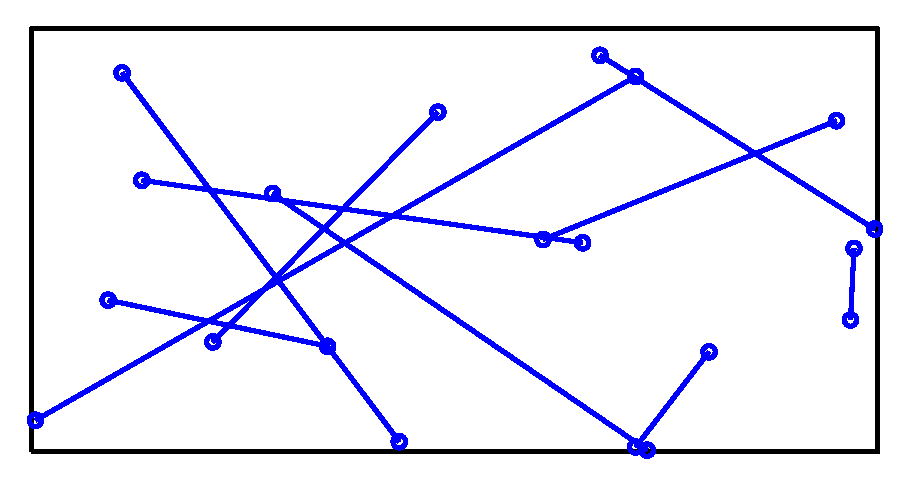
\includegraphics[width=0.4\columnwidth]{../Matlab/Plots/LinePicking_test_sim_rect_eg.eps}} 
    \hspace{6mm}
    \subfloat[\label{fig:rect_pdf}PDF of rectangle with various aspect
    ratios.]{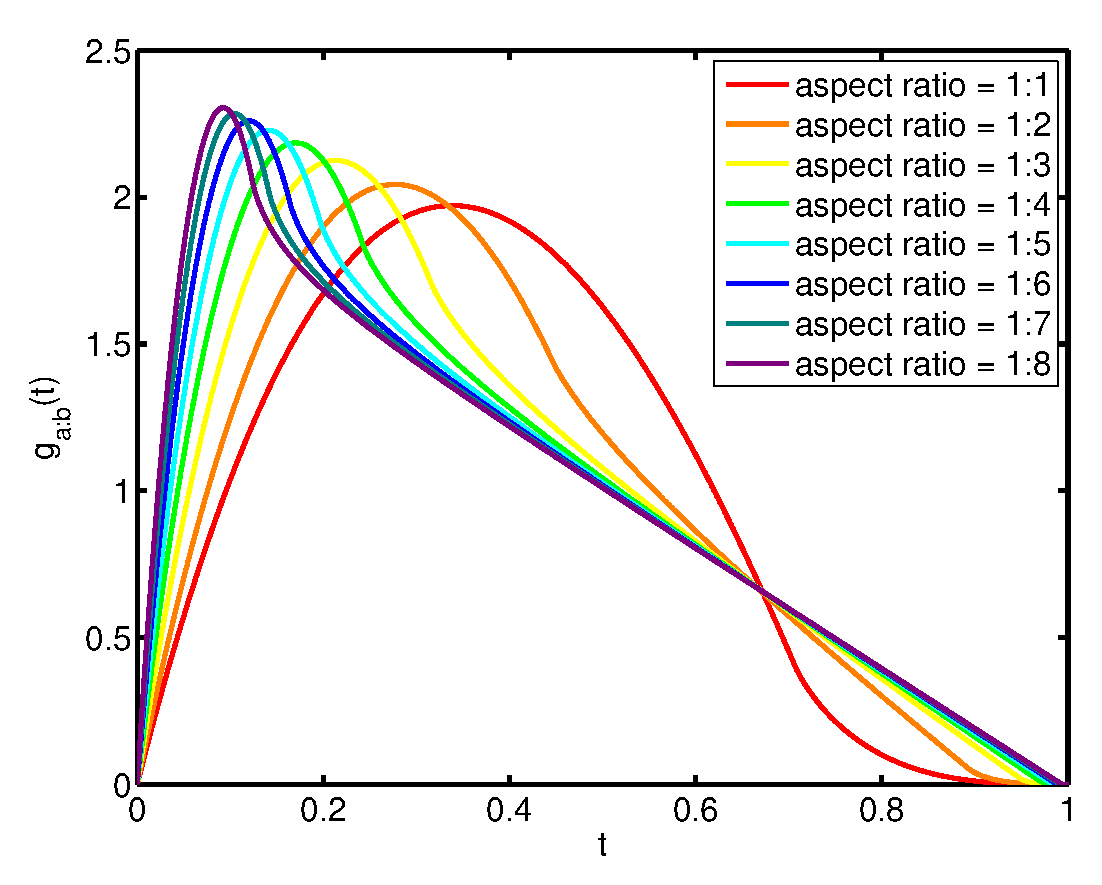
\includegraphics[width=0.48\columnwidth]{../Matlab/Plots/LinePicking_test_rect.eps}}
    \caption{The rectangle-line picking problem.}
  \end{center} 
\vspace{-4mm}
\end{figure}

\subsubsection{PDF}

The PDF for the rectangle is given in \cite[Theorem
2.4.4]{mathai_geom} and \cite[Theorem 2]{b.ghosh51:_random_rect}
\begin{equation}
  g^{\rm rect}_{a,b}(t) = \frac{4 t}{a^2 b^2} \phi_{a,b}(t),
  \label{eqn:rectangle}   
\end{equation}
where
\begin{equation}
  \phi_{a,b}(t) = \left\{
    \begin{array}{ll}
      \frac{ab \pi}{2} - (a+b) t + \frac{t^2}{2}, 
         & \mbox{ for } t \leq a, \\
      a b \sin^{-1} (a/t) - \frac{a^2}{2} - b t + b\sqrt{t^2 - a^2},
         & \mbox{ for } a \leq t \leq b, \\
      a b \left[ \sin^{-1} (a/t) - \sin^{-1} \sqrt{1 - \frac{b^2}{t^2}} \right]
        - \frac{a^2 + b^2 + t^2}{2} 
        + a\sqrt{t^2 - b^2}+ b\sqrt{t^2 - a^2},
         & \mbox{ for } b \leq t \leq \sqrt{a^2 + b^2}, \\
      0,
         & \mbox{ otherwise}, \\
    \end{array} \right. 
\end{equation}
where the rectangle has sides of length $a \leq
b$. Figure~\ref{fig:rect_pdf} shows these for various cases, chosen
such that $\sqrt{a^2 + b^2} = 1$ to allow comparison. We label these
rectangles by their aspect ratio $a: b$.

This is a rather complicated expression, but is easily evaluated
numerically.  Naldi \cite{m.naldi05:_connec_of_waxman_graph}
approximated this expression with a $\beta$ function, though given the
requirements to numerically evaluate that function there hardly seems
any advantage, though we shall see later that this would have been
completely appropriate if the region have been a circle.

\subsubsection{CDF}


\subsubsection{Moments}

